% !TeX root = index.tex
\iffalse
This chapter looks specifically at your results.
* You measured some samples. 
What values did you measure? 
Present them in a table or graph? 
How did you test whether they were good measurements? 
Were you looking to improve something? 
Are your new samples better than the old ones?

* You built a device; 
what tests did you run to make sure that it is running correctly?

* You calculated something or developed a new theory about something. 
How do you know how well it predicts? 
What tests did you run? 
What comparisons with the literature did you make?
* You coded or simulated something. 
What tests did you run to be sure it was working correctly? 

Describe what you want the reader to notice in the results. 
Give the facts, then give your analysis of the facts.
Present your graphs, figures, tables, photos, and equations needed to show what you accomplished.
Label everything clearly, using the recommendations given below in “Things to Look For”
\fi

\subsection{FPGA logic component composition}
This subsection looks at test and its results to find how much FPGA logic components each processor takes and what is composition of each part.

Test was performed with Quartus synthesis tool and viewing flow summary report. This report includes synthesised design metrics including total logic elements, registers, memory bits and other FPGA resources. Test will only look at logic elements and registers. Total number of logic elements was found out by synthesising full processors, then commenting relevant parts of code, re-synthesising and viewing changes in total logic elements. Such method may not be the most accurate, because during HDL synthesis circuit is optimised an unused connections removed. This means that more logic may be not synthesised than intended. 

There are four parts of each processor that will be tested: 
\begin{enumerate}
	\item \textbf{Common} - processor auxiliary logic that is used by both processors. It includes communication block with UART, RAM and PLL (Phase-Locked Loop, for master clock generation). 
	\item \textbf{ALU} - as described in section \ref{subsec:alu}, both processors have slightly different implementation of ALU.
	\item \textbf{Memory} - processors memory management, including stack.
	\item \textbf{Other} - reminding logic of processor that was not analysed.
\end{enumerate}

\begin{colfigure}
	\centering
	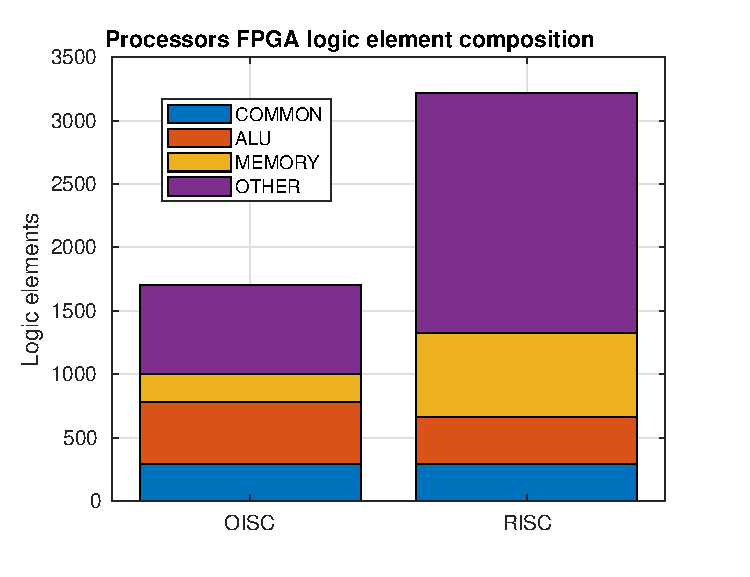
\includegraphics[width=\linewidth]{../tests/fpga_comp.eps}
	\captionof{figure}{Bar graph of FPGA logic components taken by each processor.}
	\label{fig:fpga_comp}
\end{colfigure}

Results of a test are shown in figures \ref{fig:fpga_comp} and \ref{fig:fpga_reg_comp}. Common logic uses 293 logic elements and 170 registers. OISC uses 1705 logic elements, while RISC uses 3218. Excluding common logic, OISC takes 48.3\% of RISC's logic elements.


\begin{colfigure}
	\centering
	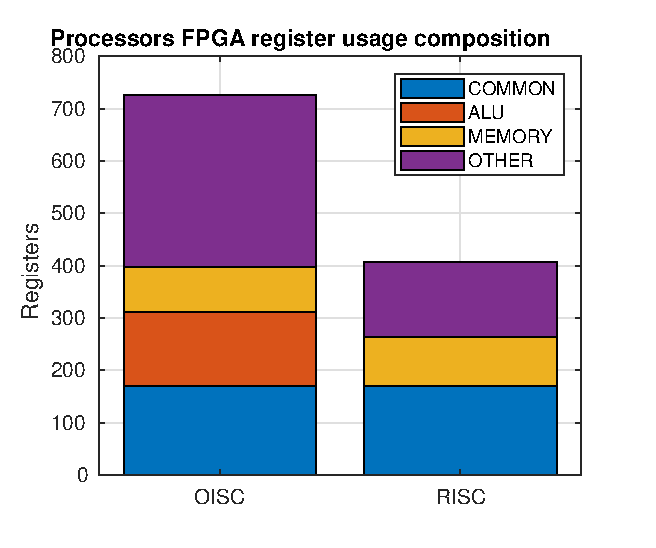
\includegraphics[width=\linewidth]{../tests/fpga_reg_comp.eps}
	\captionof{figure}{Bar graph of FPGA register resources taken by each processor.}
	\label{fig:fpga_reg_comp}
\end{colfigure}

OISC uses 726 logic elements, while RISC uses 407. Excluding common logic, OISC uses 78.4\% more registers than RISC.

Looking at composition, OISC ALU takes 30.2\% more logic gates. Looking at figure \ref{fig:fpga_reg_comp}, high number of OISC ALU registers can be observed which concludes, that higher resource usage is OISC ALU code include buffer logic.

Memory logic elements composition of OISC is only 34.4\% of RISC's and 7\% lower for register resources, comparing to RISC. This indicate that by removing memory logic for RISC, synthesis tool may removed also other parts of processor, possibly part of control block because it mostly contains combinational logic.

Other logic includes instruction decoding with ROM, register file, program counter. RISC exclusively has control block. Note that OISC uses  only three ROM memory blocks whereas RISC uses four as explained in section \ref{subsec:memory}, however this should make a minimal difference as M9K memory blocks are not included in FPGA logic element or register count. Comparing both processors, OISC has only 37\% of other logic components to RISC, however it has 2.28 times more registers. This shows a logic component - register trade-off. OISC buffer and common registers logic that connects bus require many more registers whereas RISC uses combination logic in control block in order to control same data in datapath. 

Much higher logic components in RISC can be also explained more complicated register file, ROM memory logic and program counter. All of these components has some additional logic for timing correction or additional functionality required by these blocks integration into datapath.

\subsection{Benchmark Programs}

\colorbox{yellow}{\parbox{\columnwidth}{Description of each function in benchmark to be added.}}

\subsubsection{Performance}
\colorbox{yellow}{\parbox{\columnwidth}{Data of benchmark functions timings to be added.}}

\subsubsection{Instruction composition}
This test is performed to investigate instruction composition of each function to see how similar it is between RISC and OISC processors. 
\begin{description}
	\item[$\bullet$ MOVE] - All instructions that move data around internal processor registers.
	\item[$\bullet$ ALU] - Instructions that are used to perform ALU operation.
	\item[$\bullet$ MEMORY] - Instructions that are required to send/retrieve data from system memory, except stack.
	\item[$\bullet$ STACK] - Instructions that push/pop data from memory stack.
	\item[$\bullet$ COM] - Instruction(s) that send/receive data from communication block.
	\item[$\bullet$ BRANCH] - Instructions that are used to make program branching.
	\item[$\bullet$ OTHER] - Any other instructions.
\end{description}

\begin{blockpage}
	\arrayrulecolor{black}
	\begin{tabular}{| c | p{0.65\linewidth} |} \hline 
		\rowcolor[rgb]{0.82,0.82,0.82}
		Name & Instructions \\\hline
		MOVE & \texttt{MOVE, CPY0, CPY1, CPY2, CPY3, CI0, CI1, CI2} \\\hline
		ALU & \texttt{%
			ADD, ADDI,
			SUB, SUBI,
			AND, ANDI,
			OR, ORI,
			XOR, XORI,
			DIV, MUL,
			ADDC, SUBC,
			INC, DEC,
			SLL, SRL, 
			SRA, GETAH
		} \\\hline
		MEMORY & \texttt{LWLO, LWHI, SWLO, SWHI} \\\hline
		STACK  & \texttt{PUSH, POP} \\\hline
		COM & \texttt{COM} \\\hline
		BRANCH & \texttt{BEQ, BGT, BGE, BZ, JUMP, CALL, RET} \\\hline
		\arrayrulecolor[rgb]{0,0,0}\hline
	\end{tabular}
	\captionof{table}{RISC processor instruction groups used in instruction composition test.}
	\label{tab:instr_groups_risc}
\end{blockpage}

\begin{blockpage}
	\arrayrulecolor{black}
	\begin{tabular}{| c | p{0.65\linewidth}|} \hline 
		\rowcolor[rgb]{0.82,0.82,0.82}
		Name & Destination \\\hline
		\arrayrulecolor[rgb]{0.82,0.82,0.82}
		MOVE & \texttt{REG0, REG1} \\\hline
		ALU & \texttt{ALU0, ALU1} \\\hline
		MEMORY & \texttt{MEM0, MEM1, MEM2, MEMLO, MEMHI} \\\hline
		STACK  & \texttt{STACK}\\\hline
		COM & \texttt{COMA, COMD}\\\hline
		BRANCH & \texttt{BR0, BR1, BRZ}\\\hline
		\arrayrulecolor[rgb]{0,0,0}\hline
	\end{tabular}
	\captionof{table}{OISC processor instruction desination groups used in instruction composition test}
	\label{tab:instr_groups_oisc_dst}
\end{blockpage}

\begin{blockpage}
	\arrayrulecolor{black}
	\begin{tabular}{| c | p{0.65\linewidth} |} \hline 
		\rowcolor[rgb]{0.82,0.82,0.82}
		Name & Instructions \\\hline	
		\arrayrulecolor[rgb]{0.82,0.82,0.82}	
		MOVE & \texttt{ALU0, ALU1, REG0, REG1, PC0, PC1, NULL, IMMEDIATE} \\\hline
		ALU & \texttt{ADD, ADDC, SUB, SUBC,
		AND, OR, XOR, SLL,
		SRL, EQ, GT, GE, NE,
		LT, LE, MULLO, MULHI, DIV, MOD,
		ADC, SBC, ROL, ROR} \\\hline
		MEMORY & \texttt{MEM0, MEM1, MEM2, MEMLO, MEMHI} \\\hline
		STACK  & \texttt{STACK} \\\hline
		COM & \texttt{COMA, COMD} \\\hline
		BRANCH & \texttt{BR0, BR1} \\\hline
		\arrayrulecolor[rgb]{0,0,0}\hline
	\end{tabular}
	\captionof{table}{OISC processor instruction source groups used in instruction composition test}
	\label{tab:instr_groups_oisc_src}
\end{blockpage}

Each function was ran on simulated processor, program counter and instruction been recorded into file at every cycle. File recording was done with SytemVerilog test bench, it started recording when program counter matched \texttt{.start} location and stopped when it matched \texttt{.done} location. Code shown in listings \ref{asmrisctest} and \ref{asm_oisc_test} enabled both location to be static, not depending on test function executed.

\begin{blockpage}
	\begin{lstlisting}[frame=single, caption={RISC assembly frame for executring tests}, emph={setup,start,done} label=asmrisctest]
	setup:
	JUMP .start
	.done:
	JUMP .done
	.start:
	; Setup values
	; Call function
	JUMP .done
	\end{lstlisting}
\end{blockpage}

\begin{blockpage}
	\begin{lstlisting}[frame=single, caption={OISC assembly frame for executring tests}, emph={setup,start,done} label=asm_oisc_test]
	setup:
	BR1 .start @1
	BR0 .start @0
	BRZ 0x00
	.done:
	BRZ 0x00
	.start:
	; Setup values
	; Call function
	BR1 .done @1
	BR0 .done @0
	BRZ 0x00
	\end{lstlisting}
\end{blockpage}

Each function recorded file then was further analysed and each instruction was grouped. Recorded program counter was used to find effective program space. This has been achieved by calculating unique instances of program counter and summing up instruction size for each of them. In RISC, dynamic instruction size has been taken into account. 

Results or each function composition are represented in figure \ref{fig:instr_comp}. 
\begin{figure*}[t]
	\centering
	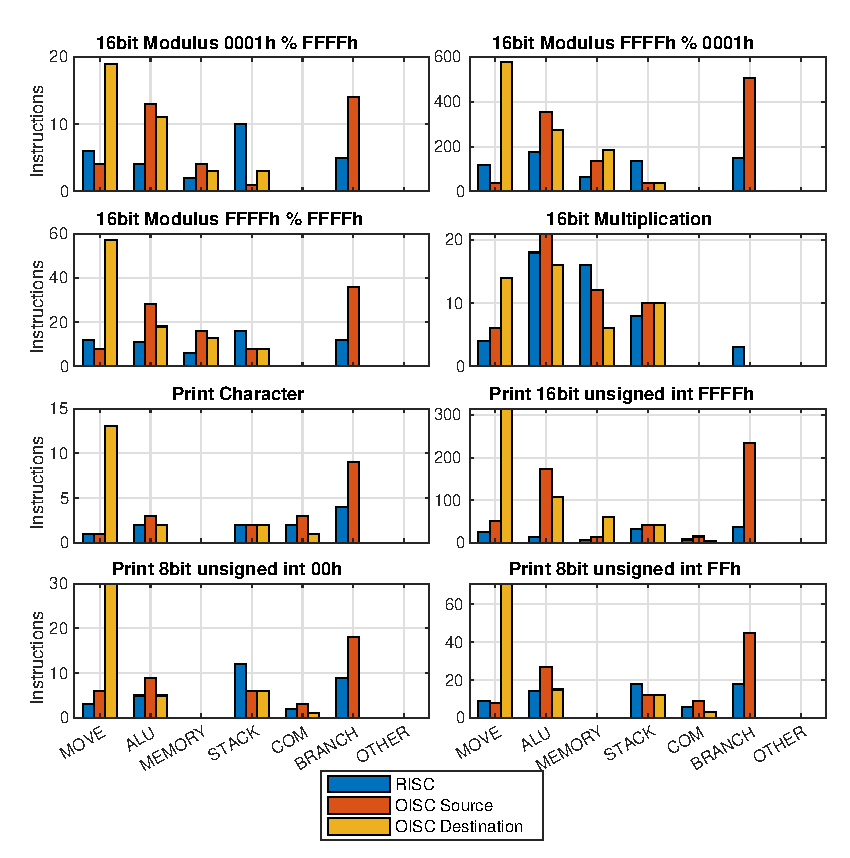
\includegraphics[width=\linewidth]{../tests/instr_comp.eps}
	\caption{Graph of instruction composition for every benchmark program.}
	\label{fig:instr_comp}
\end{figure*}

\subsubsection{Program space}

Figure \ref{fig:program_size} represents effective program size for each test function. Effective program size only includes instruction that been executed depending on argument, meaning that it does not fully represent complete function. A specific argument might cause branching and skipping some function code which would not be added to effective program size. In this test, the main objective is to look difference in instruction size required to execute the same function, therefore not representing full program size is not relevant. 
\begin{colfigure}
	\centering
	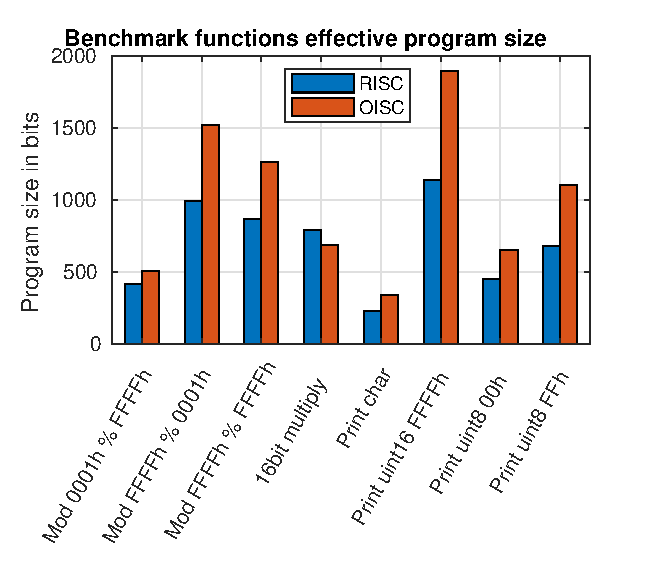
\includegraphics[width=\linewidth]{../tests/program_size.eps}
	\captionof{figure}{Bar graph showing effective size in bits each benchmark function is taking in program memeory.}
	\label{fig:program_size}
\end{colfigure}

\subsection{Maximum clock frequency}
\colorbox{yellow}{Description to be added.}


